

\section{Methodology}
\label{sec:method}

Think-on-Graph 3.0 (ToG-3) introduces a novel \emph{Multi-Agent Context Evolution and Retrieval (MACER)} framework for open-domain question answering. 
% Unlike prior ToG systems that rely on pre-existing, monolithic knowledge graphs (e.g., Freebase, Wikidata) or static GraphRAG methods that construct a fixed graph from a corpus in a single pass, ToG-3 employs a synergistic set of LLM agents. These agents—Constructor, Retriever, Reflector, and Response—collaborate in a single-loop, provably convergent process to (i) build an incrementally refinable heterogeneous graph index, (ii) decompose complex questions into a sequence of adaptive sub-queries, and (iii) synthesize faithful, step-by-step answers. 
% Crucially, we formalize the iterative retrieval–reflection process as a Markov Decision Process (MDP) and leverage recent advances in implicit gradient theory~\citep{dherin2025learning} to prove that our method performs stochastic gradient descent on the LLM's implicit loss landscape, guaranteeing convergence.

\subsection{Problem Formulation}
\label{subsec:problem}

Let $\mathcal{D}=\{d_i\}_{i=1}^N$ be a text corpus. The objective is to answer a user query $q$ with an answer $a^*$ that is both accurate and \emph{faithful} to the source corpus, derived from a \emph{minimal, sufficient subgraph} $\mathcal{G}^*_q$ of a heterogeneous graph $\mathcal{G}$ constructed from $\mathcal{D}$:
\begin{align}
    \mathcal{G}^*_q = \operatorname*{argmin}_{\mathcal{G}' \subseteq \mathcal{G}} |\mathcal{G}'| \quad \text{subject to} \quad \texttt{Suff}(q, \mathcal{G}') = 1,
\end{align}
where $\texttt{Suff}(\cdot, \cdot) \in \{0,1\}$ is an function judging the sufficiency of a subgraph for answering the query.

Existing methods face a critical dilemma: \textbf{(1)} Systems like ToG-1 or 2 rely on high-quality, pre-constructed KGs, limiting their applicability to private or specialized domains. \textbf{(2)} Corpus-based GraphRAG methods (e.g., GraphRAG, LightRAG) build a static graph from $\mathcal{D}$ in one go. Their performance is bottlenecked by the quality of this initial graph, which in turn depends heavily on the capability of the LLM used for information extraction. 
% Using powerful LLMs (e.g., GPT-4) is computationally expensive and often infeasible for on-premise deployment due to API constraints, while smaller, local LLMs ($\leq$32B parameters) suffer from high triplet extraction failure rates, coarse entity resolution, and low recall, leading to suboptimal retrieval and subsequent hallucinations.

% ToG-3 overcomes these limitations through a dynamic, multi-agent process that \emph{iteratively refines} the retrieved evidence context ($\mathcal{G}_k$) in direct response to the reasoning needs of the query, mitigating the shortcomings of the initial static graph built by a small LM.

\subsection{Heterogeneous Graph Index: Schema and Construction}
\label{subsec:index-graph}

\subsubsection{Node and Edge Schema}
The Constructor Agent builds a heterogeneous graph $\mathcal{G}=(\mathcal{V},\mathcal{E})$ with three node types:
\begin{itemize}
    \item \textbf{Chunks} ($\mathcal{C}$): Sentence-level text passages from the corpus. 
    % $|\mathcal{C}|$ is approximately $3N$.
    \item \textbf{Triplets} ($\mathcal{T}$): Semantic triples $(s, p, o)$ extracted from chunks, annotated with entity and relation types ($\texttt{type}_s$, $\texttt{type}_p$, $\texttt{type}_o$).
    \item \textbf{Communities} ($\mathcal{M}$): Summaries of entity clusters obtained via Leiden clustering on the entity co-occurrence graph, each condensed into an abstract.
\end{itemize}
Edges are defined by three type relations:
\begin{itemize}
    \item \textbf{$\textsc{OpenRel}(s, p, o)$}: Connects entities $s$ and $o$ via predicate $p$ extracted by the LLM, forming an open-domain semantic triple.
    \item \textbf{$\textsc{MentionedIn}(t, c)$}: Connects a triplet $t$ to the chunk $c$ from which it was extracted.
    \item \textbf{$\textsc{SummaryFor}(m, e)$}: Connects a community summary node $m$ to an entity $e$ that belongs to that community.
\end{itemize}
This unified schema allows both fine-grained (chunk/triplet) and high-level (community) information to be retrieved seamlessly within a single vector space, effectively addressing the local/global retrieval dichotomy of prior GraphRAG systems.

\subsubsection{Offline Index Construction}
\label{subsubsec:offline-build}
Algorithm~\ref{alg:offline-construct} in Appendix.~\ref{appendix:algs} details the one-time construction of the universal index $\mathcal{G}$. A key design choice is the use of a single frozen encoder $E_\theta$ (e.g., jina-mebedding-v3~\citep{sturua2024jinaembeddingsv3}) to embed all nodes—regardless of type—into a unified 1024-dimensional dense vector space. This enables efficient vector search across all node types during retrieval.

% \begin{figure}
%     \centering
%     \includegraphics[width=0.95\linewidth]{figs/graph_construct.pdf}
%     \caption{\textbf{ToG-3 Offline Universal Index Construction.}
% Given the full corpus, the Constructor Agent (i) slices documents into sentence-level chunks, (ii) extracts typed entity-relation triplets via a lightweight local LLM, and (iii) performs Leiden clustering to generate community summaries.
% The resulting heterogeneous graph unifies chunks, triplets, and community nodes in a single dense vector space, enabling later query-time refinement.}
%     \label{fig:graph_construct}
% \end{figure}


\subsection{The MACER Process: Multi-Agent Context Evolution and Retrieval}
\label{subsec:macer-process}


The core of ToG-3 is the online MACER loop (Algorithm~\ref{alg:tog3-full}), an iterative process of retrieval, generation, and reflection that dynamically evolves the context subgraph $\mathcal{G}_k$. We formalize this process as an episodic Markov Decision Process (MDP) $\mathcal{M}=(\mathcal{S}, \mathcal{A}, P, r)$.
% (\mathcal{S}, \mathcal{A}, P, r, \gamma)$ to rigorously analyze its convergence properties and agent interactions.

\begin{figure*}
    \centering
    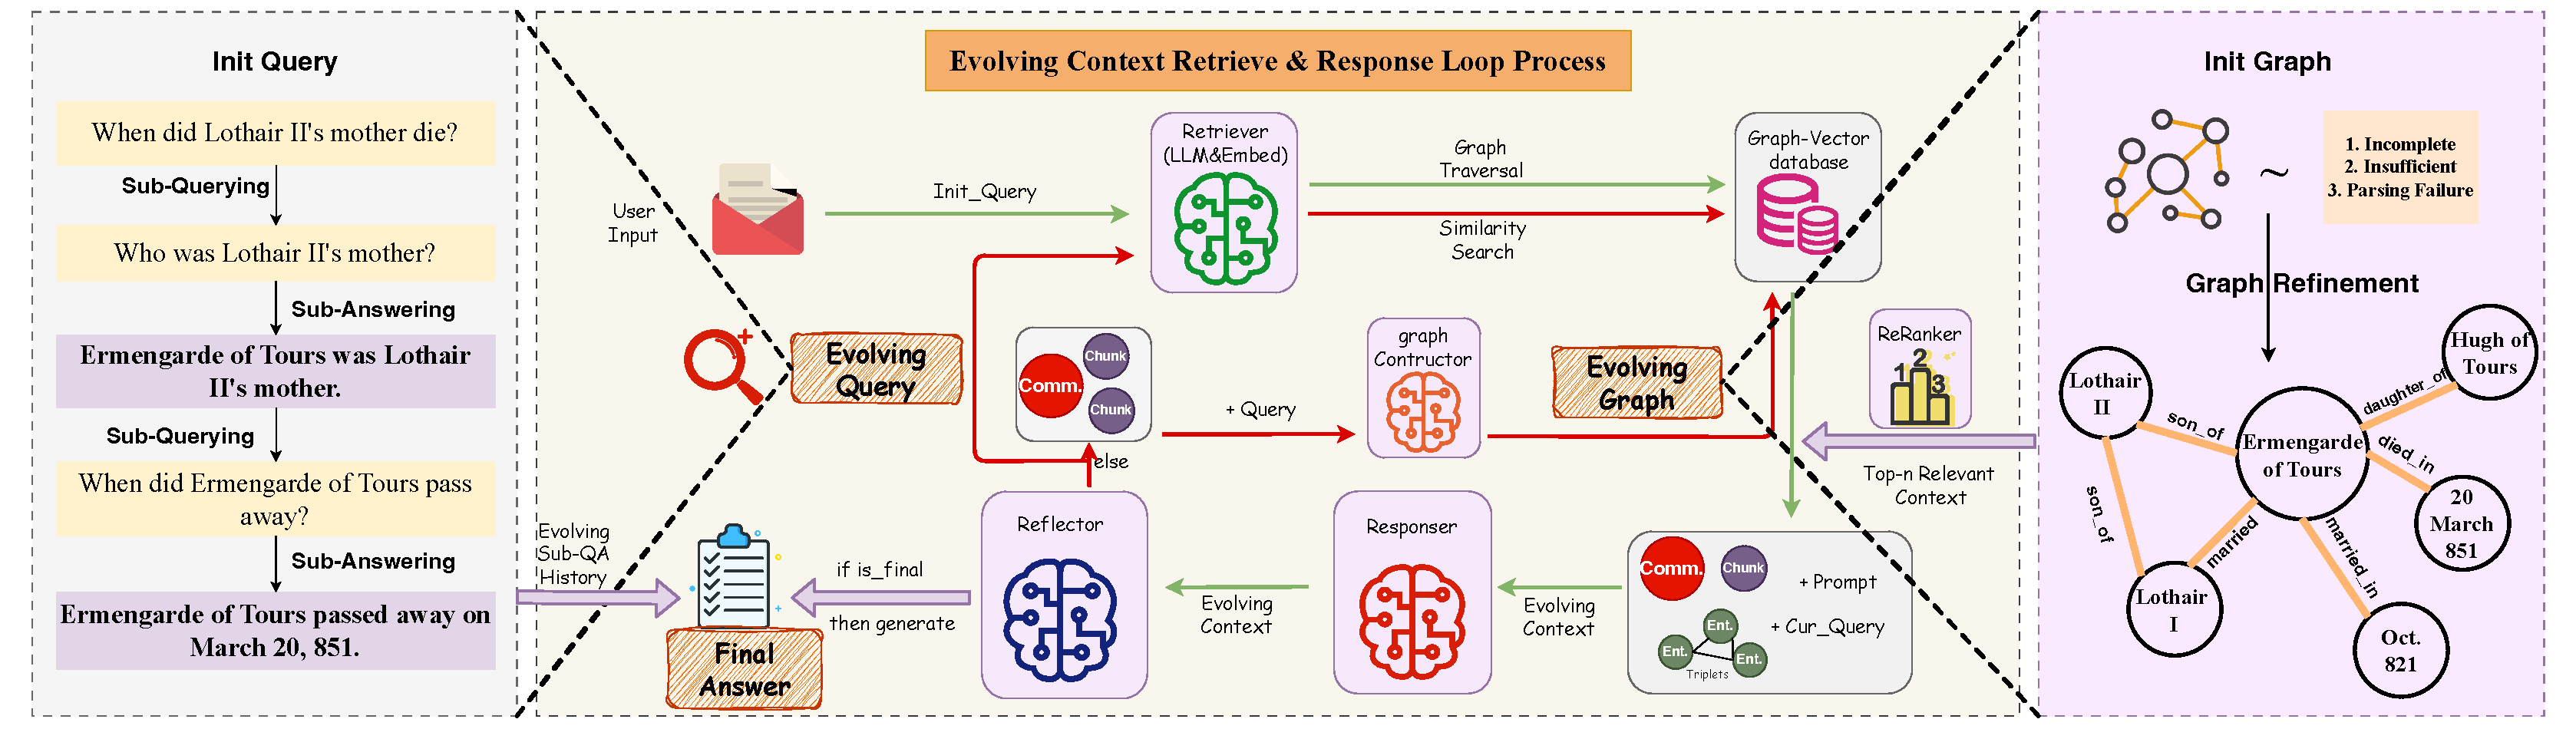
\includegraphics[width=1.0\linewidth]{figs/retrieve_response.pdf}
    \caption{\textbf{Multi-Agent Dual-Evolving Context Retrieval-Response Loop.}
The Retriever fetches an initial chunk–triplet–community subgraph and the Reranker reranks and selects the top-n most relevant pieces of evidence..
The Response Agent produces an answer; the Reflector Agent judges sufficiency (reward=1/0).
If insufficient (reward=0), the Reflector evolves the query into sub-queries while the Constructor evolves the subgraph (sub-graph refinement).
The loop repeats until the context becomes sufficient or the horizon is reached, after which the Response Agent synthesizes the final answer from the full trajectory.}
    \label{fig:retrive_response}
\end{figure*}

% \subsubsection{MDP Formalization of the MACER Loop}

\paragraph{State Space ($\mathcal{S}$)}: At each step $k$, the state $s_k = (q, \mathcal{G}_k, \mathcal{H}_k)$ captures the complete reasoning context, including the original query $q$, the current evidence subgraph $\mathcal{G}_k$ retrieved by Retriever Agent $\pi_{\text{ret}}$ and reranked by Reranker Agent $\pi_{\text{rer}}$, and the trajectory history $\mathcal{H}_k = {(q'_i, a_i, r_i, \mathcal{G}i)}_{i=0}^{k-1}$ of all previous sub-queries, answers, rewards, and sub-graphs.

\paragraph{Action Space ($\mathcal{A}$)}: The Reflector Agent $\pi_{\text{ref}}$ serves as the policy network. Its action $a_k$ at state $s_k$ is either to generate a targeted refinement sub-query $q'_k$ (to continue the reasoning process) or to output the $\textsc{stop}$ action (to terminate the episode).

\paragraph{Reward Function ($r$)}: Upon the Response Agent generating an answer $a_k$, the Reflector immediately provides a sparse, binary reward $r_k$:
\begin{align}
    r_k = \begin{cases}
        1 & \text{if } \texttt{Suff}(q, \mathcal{G}_k, a_k) = 1\\
        0 & \text{otherwise.}
    \end{cases}
\end{align}
This reward signal is produced by the Reflector Agent to determine if the current context evidence is sufficient to answer the user's query. 
% directly dictates the termination condition and guides the refinement process.

\paragraph{Transition Dynamics ($P$)}
Given the current state $s_k$ and an action $a_k$ (which corresponds to issuing a sub-query $q'k$), the transition to the next state $s_{k+1}$ occurs deterministically according to the following update rules:
% \begin{equation}
% \mathcal{G}_{k+1} = \pi_{\text{const}}(q'_k, \mathcal{G}_k)
% \end{equation}
The constructor agent $\pi_{\text{const}}$ applies the transition operator using the generated sub-query $q'_k$ and the current graph state $\mathcal{G}_k$ to produce an updated graph $\mathcal{G}_{k+1}$. 
This step including iterative sequence of \emph{evolving queries} and \emph{evolving sub-graphs} reflects the structural evolution of the graph based on the agent's reasoning action, formally defined by the recurrence:
\begin{align}
    q'_{k} &= \pi_{\text{ref}}^{\text{evolve}}(q, \mathcal{G}_k), \\
    \mathcal{G}_{k+1} &= \pi_{\text{const}}^{\text{evolve}}(q'_k, \mathcal{G}_k),
\end{align}
% where at each step $k$, the Reflector Agent first generates an evolved sub-query $q'_k$ targeting the identified knowledge gaps in the current context $\mathcal{G}k$. The Constructor Agent then evolves the sub-graph by performing targeted refinement—expanding with relevant nodes, optionally re-extracting triplets from new chunks, and pruning irrelevant information—to produce $\mathcal{G}{k+1}$. 

The action history $\mathcal{H}_{k+1}$ is augmented with a new tuple recording the executed sub-query $q'_k$, the corresponding action $a_k$, the reward $r_k$ received, and the resulting graph state $\mathcal{G}_{k+1}$. This ensures a comprehensive trace of the reasoning trajectory, which is essential for credit assignment and subsequent learning.

\begin{equation}
\mathcal{H}_{k+1} = \mathcal{H}_k \cup { (q'_k, a_k, r_k, \mathcal{G}_{k+1}) }
\end{equation}
\begin{equation}
 a^* \gets \pi_{\text{resp}}^{\text{final}}(q, \mathcal{H}_k)
\end{equation}

The complete MACER process, now cast as an MDP, is summarized in Algorithm~\ref{alg:tog3-full}. The loop continues until the Reflector's policy $\pi_{\text{ref}}$ outputs the $\textsc{stop}$ action (via $r_k=1$) or a maximum horizon $K$ is reached. The final answer $a^*$ is synthesized from the full trajectory $\mathcal{H}_k$ of states and actions, ensuring faithfulness to the evolved evidence.
This MDP formulation provides the formal foundation for establishing the convergence of the MACER process under mild assumptions, as detailed in Appendix.~\ref{appendix:theory_support}.
% where we show its equivalence to implicit gradient descent.
This iterative refinement allows ToG-3 to start from a potentially weak initial graph but \emph{specialize} it towards the reasoning path of the specific query, converging on a high-quality evidence subgraph $\mathcal{G}^*_q$. 
This evolving and refinement mechanism alleviate the three fundamental weaknesses of small LMs in static GraphRAG, including incomplete triplet recall, insufficient knowledge details and high parsing failure of LLMs' output, as mentioned in Section~\ref{sec:intro}. 

% This evolving and refinement mechanism provides three crucial advantages within the MDP framework:
% \textbf{Enhanced Recall}: The optional \emph{re-extraction} phase applies the triplet extractor to newly retrieved chunks, mitigating the low recall of the initial offline extraction by the small LM.
% \textbf{Targeted Exploration}: The \emph{expansion} phase retrieves nodes relevant to the specific sub-query $q'_k$, enabling the MDP to explore the graph space in a targeted manner.
% \textbf{Noise Reduction}: The \emph{contraction} phase prunes irrelevant nodes, increasing the signal-to-noise ratio in the state representation $s_k$ and leading to more reliable reward signals.
% This process directly alleviate the three fundamental weaknesses of small LMs in static GraphRAG, including incomplete triplet recall, insufficient knowledge details and high parsing failure of LLMs' output, as mentioned in Section~\ref{sec:intro}. 

% In summary, the ToG-3 methodology presents a principled framework for open-domain question answering that fundamentally advances beyond existing graph-based retrieval approaches. By introducing the Multi-Agent Context Evolution and Retrieval (MACER) process, we transform static graph retrieval into a dynamic, iterative reasoning loop formalized as a Markov Decision Process. Our key innovation lies in the synergistic operation of four specialized agents that collectively construct a universal heterogeneous graph index and perform query-aware subgraph refinement through targeted expansion, re-extraction, and contraction operations. This approach effectively mitigates the limitations of small language models in knowledge extraction while eliminating the dependency on pre-existing knowledge bases. The theoretical grounding of our framework in implicit gradient theory provides formal convergence guarantees, ensuring that the iterative refinement process provably converges to a minimal sufficient evidence subgraph. Together, these contributions establish ToG-3 as a robust, efficient, and theoretically sound methodology for complex question answering across diverse domains.






